\chapter{总结}

\section{项目中遇到的问题及解决方法}
\subsection{后端调试过程中遇到的问题}

在后端调试过程中,遇到一些程序上的错误,如图8-1,8-2所示
\begin{figure}[htbp]
	\centering
	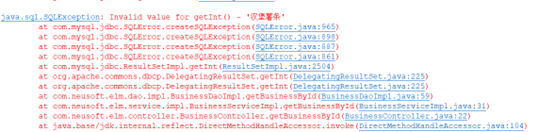
\includegraphics[width=0.8\textwidth]{pb1}
	\caption{类型不匹配问题}\label{fig:8.1}
	\vspace{\baselineskip}
\end{figure}

\begin{figure}[htbp]
	\centering
	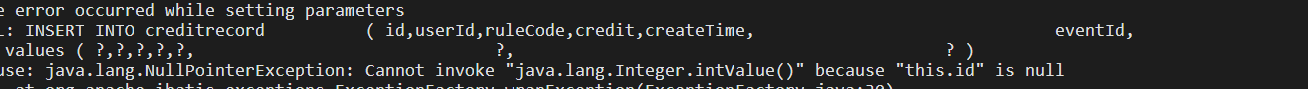
\includegraphics[width=0.8\textwidth]{pb2}
	\caption{插入值为空}\label{fig:8.2}
	\vspace{\baselineskip}
\end{figure}

解决方法:上述问题是程序运行上出现的错误,通过查询报错信息,找到出错位置,并分析数据包找出出错的原因,最终改掉程序上的错误。

\subsection{程序性能上的缺陷}
\subsubsection{问题}
在进行压力测试的时候,暴露出了挺多性能问题,如图8-3,8-4所示

\begin{figure}[htbp]
	\centering
	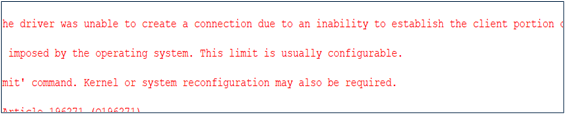
\includegraphics[width=0.8\textwidth]{pbmysql}
	\caption{mysql查询大量数据异常}\label{fig:8.3}
	\vspace{\baselineskip}
\end{figure}

\begin{figure}[htbp]
	\centering
	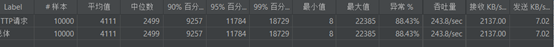
\includegraphics[width=0.8\textwidth]{pbredis}
	\caption{请求异常率过高}\label{fig:8.4}
	\vspace{\baselineskip}
\end{figure}

\subsubsection{解决方案}
第一个问题是因为默认情况下,Windows允许用于使用5000个临时TCP端口,如果使用临时连接会导致临时端口消耗过快,所以我们通过建立连接池,

节省资源开销,也就是通过池化技术优化性能,节约开销。

第二个问题是因为高并发情况下服务器无法在短时间内处理数量如此巨大的请求,这是难以避免的问题,因为服务器性能有限,所以我们通过线程池,以及做mysql缓存,提供线程池数量,尽量优化程序的性能,有效减少在高并发下的错误率。

\subsection{前后端部署上的问题}
\subsubsection{问题}
在将前后端合并部署到服务器过程中,遇到了如下图的问题

\begin{figure}[htbp]
	\centering
	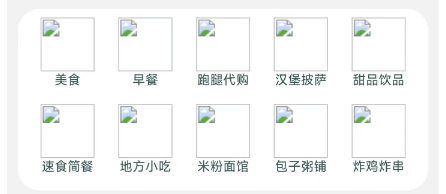
\includegraphics[width=0.8\textwidth]{pb3}
	\caption{图片加载不出}\label{fig:8.5}
	\vspace{\baselineskip}
\end{figure}

同时还遇到了能够访问前端主页,但点击切换网址时,无法跳转,前端请求被后端拒绝的问题。

\subsubsection{解决方案}
第一个问题,是因为在第一次前后端交互时,将springboot和vue打包成一个jar包运行,图片路径问题难解决。所以我们更换方式,通过nginx运行前端,单独将后端打包成jar包运行,前端被点击时会自动将消息发送给后端,这样分开运行解决了前后端复杂的交互问题。

第二个问题通过上网查看,发现是因为端口防火墙的问题。后端8081的监听端口开启了防火墙,阻塞了前端发来的HTTP请求,关闭防火墙后前后端得以正常交互。
\section{项目开发过程}
\subsection{项目共享仓库}
我们对于本实践项目使用 GITHUB 进行仓库共享,让每一名组员可以在该仓库上进行代码的修改以及同步,大幅度增加实践效率。通过以下网址,可以游览到本项目的共享仓库页面:https://github.com/stainsatin/elm
\begin{figure}[htbp]
    \centering
    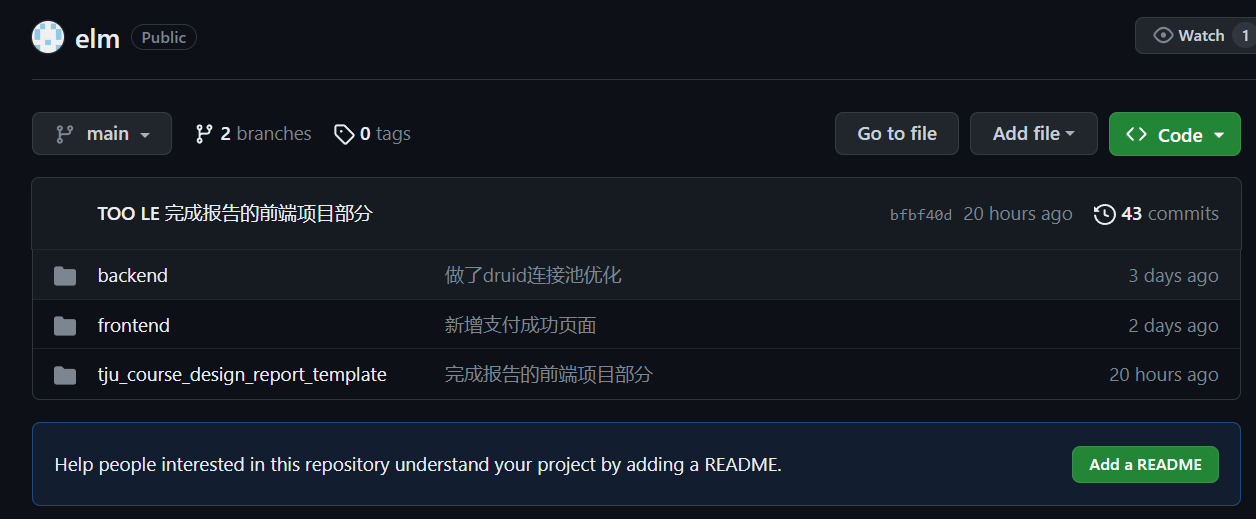
\includegraphics[width=0.8\textwidth]{githubmain}
    \caption{GITHUB 共享仓库页面}\label{fig:githubmain}
    \vspace{\baselineskip}
\end{figure}

本次实践项目的共享仓库于 8 月 23 日创建,仓库里的成员包括我们每一名组员。如上图~\ref{fig:githubmain}~所示,仓库里的内容包括本次实践项目的前端、后端与实践报告的目录,且我们每一名组员都在此共享仓库上进行了多次代码的复制和提交。经过三个星期的项目开发,以下是我们的共享仓库数据视图,如图~\ref{fig:commit}~至图所示:

\begin{figure}[htbp]
    \centering
    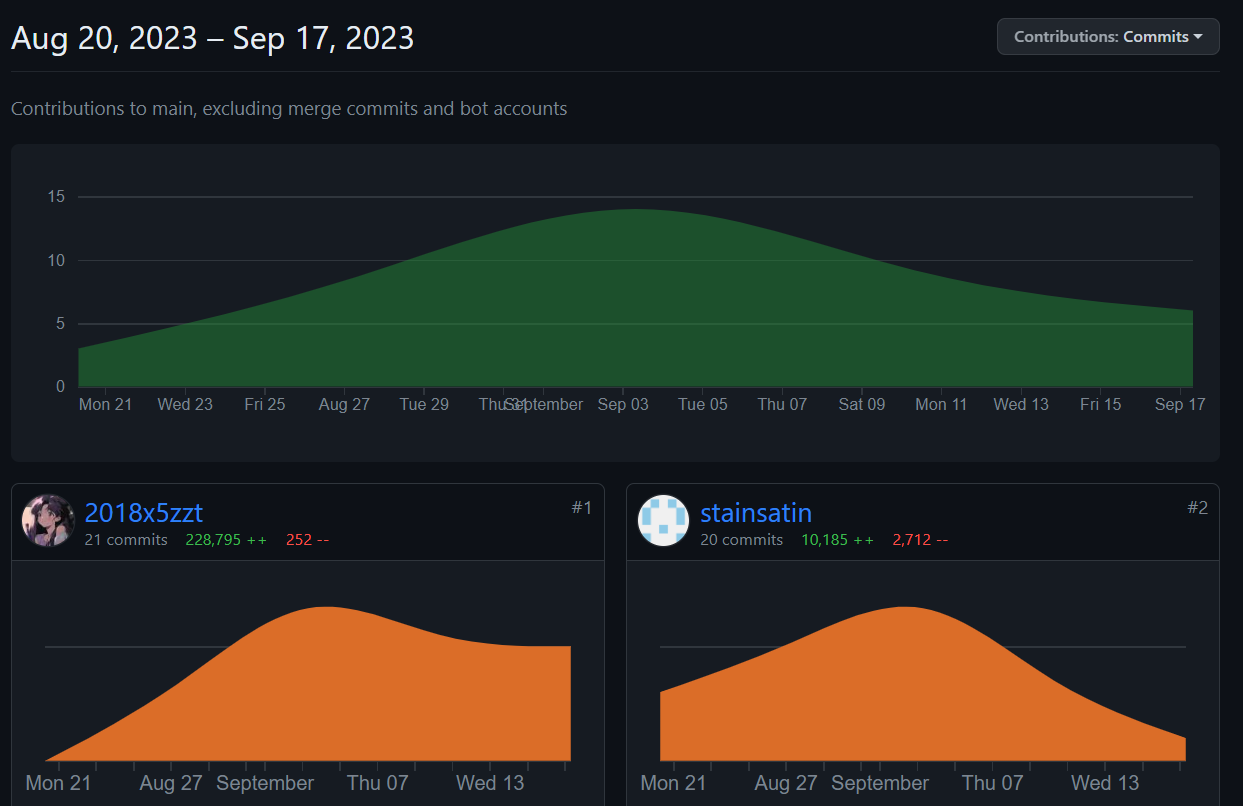
\includegraphics[width=0.7\textwidth]{commit}
    \caption{GITHUB 共享仓库提交视图}\label{fig:commit}
    \vspace{\baselineskip}
\end{figure}
\begin{figure}[htbp]
    \centering
    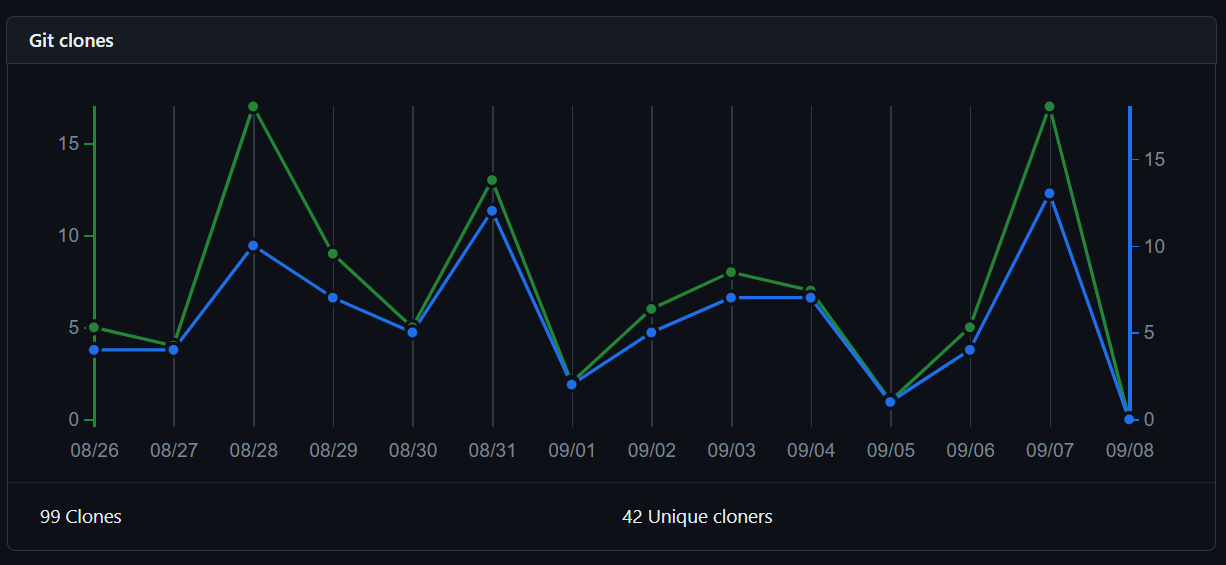
\includegraphics[width=0.8\textwidth]{clone}
    \caption{GITHUB 共享仓库复制视图}\label{fig:clone}
    \vspace{\baselineskip}
\end{figure}
\begin{figure}[htbp]
    \centering
    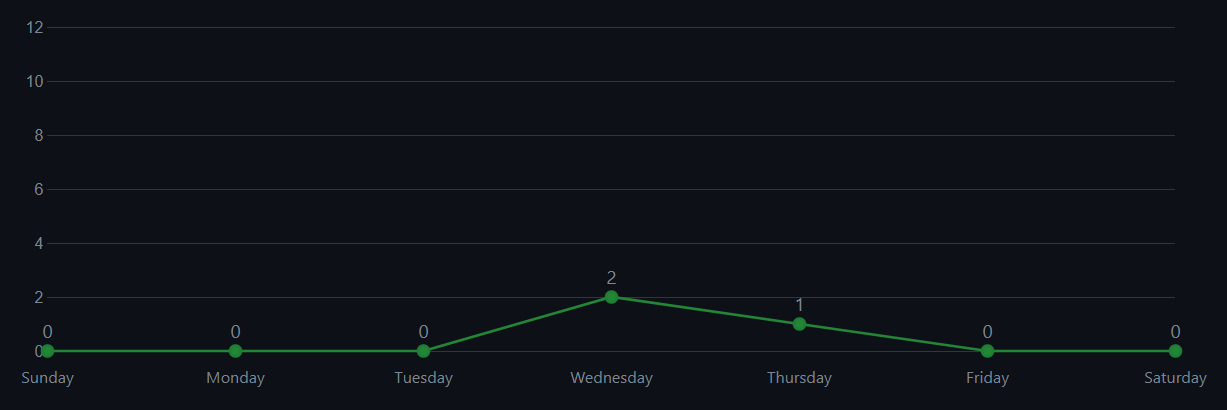
\includegraphics[width=0.8\textwidth]{week1commit}
    \caption{GITHUB 共享仓库第一周提交次数视图}\label{fig:week1commit}
    \vspace{\baselineskip}
\end{figure}
\begin{figure}[htbp]
    \centering
    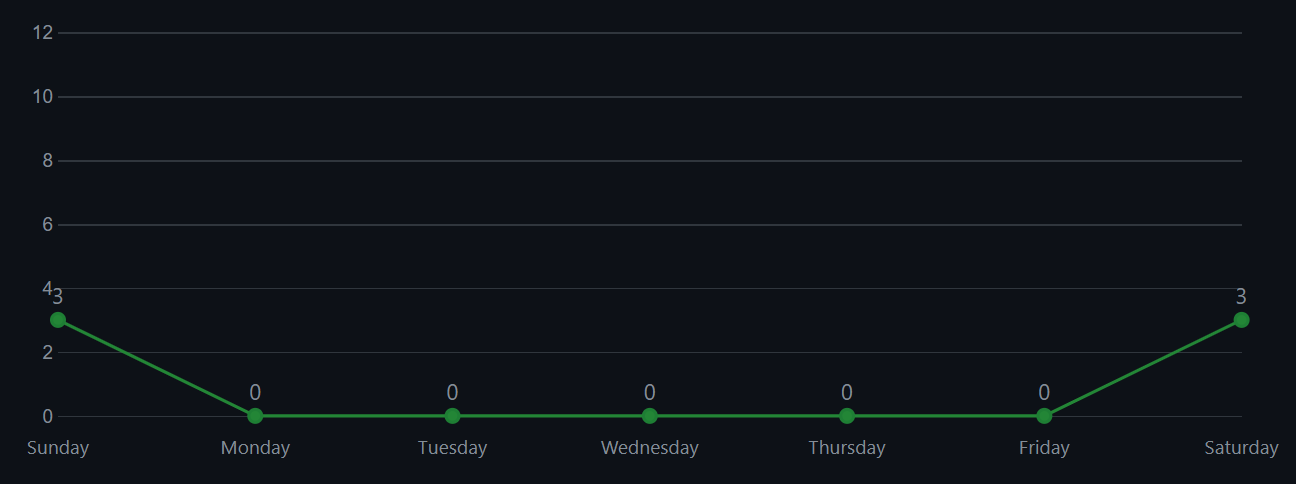
\includegraphics[width=0.8\textwidth]{week2commit}
    \caption{GITHUB 共享仓库第二周提交次数视图}\label{fig:week2commit}
    \vspace{\baselineskip}
\end{figure}
\begin{figure}[htbp]
    \centering
    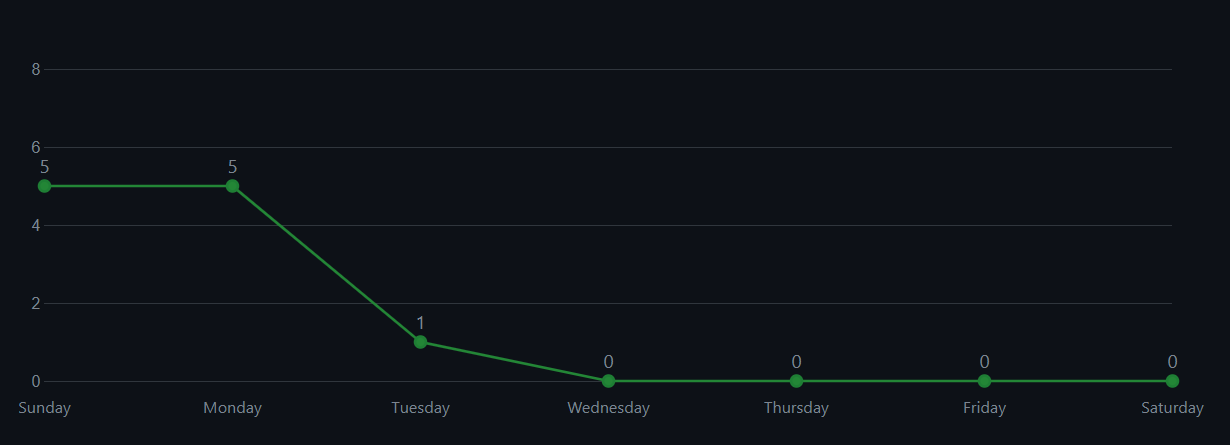
\includegraphics[width=0.8\textwidth]{week3commit}
    \caption{GITHUB 共享仓库第三周提交次数视图}\label{fig:week3commit}
    \vspace{\baselineskip}
\end{figure}
\begin{figure}[htbp]
    \centering
    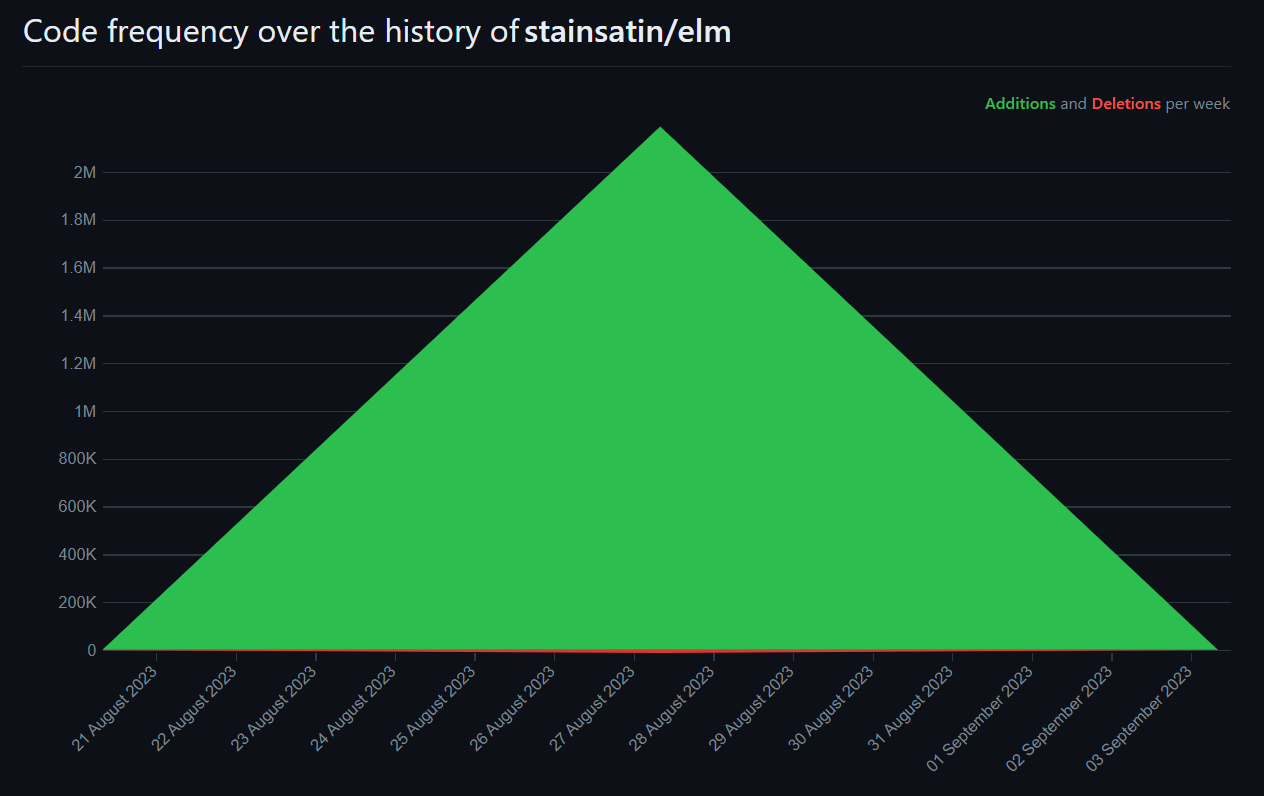
\includegraphics[width=0.7\textwidth]{codefrequency}
    \caption{GITHUB 共享仓库代码频率视图}\label{fig:codefrequency}
    \vspace{\baselineskip}
\end{figure}

\section{开发总结}
总的来说,这是一个比较复杂的软件项目。涉及到JAVAEE,javaweb,springboot,css,vue等一系列网页开发的技术,同时我们也尽量将自己学到的新技术如redis,密码学,AI相关的知识运用到这个项目当中。项目工程量比较大,同时还需要书写报告和进行汇报展示,时间比较紧。

在这样的情况下,我们四位小组成员分工明确,通过前后端分离式的开发过程,这样让自己在开发过程中,不会受别人进度太多制约,可以较为顺利完成自身的开发部分。在交互,测试的过程中,我们遇到了各种各样的问题,这些问题我们也能够准确找到问题出现的地方,知道这部分问题是由谁负责完成。大家积极配合彼此工作,才能让项目比较顺利的进行下去。

在整个项目开发过程中,每个成员都做出了重要的贡献。大家分工明确,对自己所做的部分认真负责,同时在某些阶段,当部分组员任务较重时,大家也会主动去分担任务缓解彼此压力。我们每个人都发挥自己所长,为项目做出贡献。

总的来说,这是一次收获颇丰的实践经历。通过这次软工时间,我们学会的很多网页开发的技术,项目管理的经验,也锻炼了在面对复杂问题,出现意外情况时钻研思考,独立解决问题的能力。另外我们也培养了团队成员间积极沟通,配合,团结协作的能力。相信这次宝贵的经验能让我们运用在后续在软件工程专业的学习过程中。

